% Keep spaces inside \code{...} (e.g. "POST /api/donations"); the class loads
% url through hyperref, so the options must be registered first.
\PassOptionsToPackage{obeyspaces,spaces}{url}
\documentclass{tietreport}

% Import images
\usepackage{graphicx}

% Bibliography configuration
\usepackage[
  date=year,
  style=alphabetic,
  backend=biber,
  sorting=nty,
  maxnames=5,
  minnames=3,
  maxalphanames=4,
  minalphanames=3,
  backref=true,
  doi=false,
  isbn=false,
  url=false,
  eprint=false
]{biblatex}
\addbibresource{references.bib}

%% --------------------------------------------------
%% Report-specific additions (content helpers only;
%% page layout, headers and headings come from
%% tietreport.cls unchanged)
%% --------------------------------------------------
\usepackage{array}
\usepackage[inline]{enumitem}

% fancyhdr asks for at least 14.5pt with 12pt text; the class leaves 12pt.
\setlength{\headheight}{14.5pt}

% First-level bullet from the math font (Type 1 everywhere) rather than the
% text-companion glyph, which needs cm-super to avoid a bitmap font locally.
\renewcommand{\labelitemi}{$\bullet$}

% Identifiers from the code base, set in typewriter and
% allowed to break after an underscore, dot or slash.
\DeclareUrlCommand\code{\urlstyle{tt}}
\makeatletter
\g@addto@macro{\UrlBreaks}{\do\_\do\.\do\/}
\makeatother

\newcolumntype{L}[1]{>{\raggedright\arraybackslash}p{#1}}

% Float placement: let medium tables sit in the text instead of on
% near-empty float pages (placement only; no change to formatting).
\renewcommand{\topfraction}{0.85}
\renewcommand{\bottomfraction}{0.5}
\renewcommand{\textfraction}{0.1}
\renewcommand{\floatpagefraction}{0.75}
\setcounter{topnumber}{3}
\setcounter{totalnumber}{4}

% Let a page end short rather than stretch paragraph gaps to fill it.
\raggedbottom
\setlength{\emergencystretch}{2.5em}
\renewcommand{\arraystretch}{1.18}

%% ==================================================
%% CUSTOMIZE THESE FIELDS FOR YOUR PROJECT
%% ==================================================

% Course/Lab header
\TitlePageHeader{%
  UCS503P - Software Engineering Project%
}

% Main project title
\ProjectTitle{%
  MID-TERM REPORT%
}

% Subtitle or project description
\ProjectSubTitle{%
  {\Large\bfseries FoodLink}\\[0.25cm]
  A Coordination Platform for Surplus Food Redistribution%
}

% Student information (up to 4 students)
\author{%
  \texttt{1024030909} Rishi Garg \\
  \texttt{1024030906} Aayushi Sud \\
  \texttt{1024031166} Himanshi Singla \\
  \texttt{1024030956} Yugam Heer \\[0.3cm]
  {\normalsize
  \texttt{rgarg8\_be24@thapar.edu} \quad
  \texttt{asud\_be24@thapar.edu} \\
  \texttt{hsingla1\_be24@thapar.edu} \quad
  \texttt{yheer\_be24@thapar.edu}}%
}

% Group number, degree, year, program
\TitlePageSubText{%
  Group: \texttt{3C64} BE Third Year, CSE%
}

% Faculty advisor/guide name
\AdvisorName{%
  Reaya Grewal%
}

% Evaluation period and department info
\TitlePageFooterText{{%
    \large Mid-Semester Evaluation \\[0.2cm]
    \bfseries Computer Science and Engineering
    Department%
  } \\[0.15cm]
  Thapar Institute of Engineering and Technology,
  Patiala%
}

%% ==================================================

\begin{document}

% Generate title page
\maketitle

% Table of contents (auto-generated from chapters)
\tableofcontents

% Restore these two lines if the evaluation requires the front-matter lists
% (they add about two pages):
% \listoffigures
% \listoftables

% ===== CHAPTER 1: INTRODUCTION =====
\chapter{Introduction}
\label{ch:introduction}

\section{Background and Context}
\label{sec:background}

Institutional kitchens such as college messes, hostel canteens, bakeries and
banquet halls routinely finish a service with edible food left over. At the same
time, shelters and community kitchens nearby are short of meals. Food waste is a
recognised problem at every scale~\cite{unepFoodWaste2024}. For a campus or a
tier-2/3 city, however, the binding constraint is rarely supply. It is
\emph{coordination under a deadline}: cooked food is safe for only a few hours,
and informal phone calls often outlast that window.

FoodLink is a web platform that brings every party to a handover into one tracked
workflow. A \textbf{donor} posts surplus food. An administrator verifies each
\textbf{recipient organisation} (an NGO or community kitchen) before it can
receive food. A \textbf{volunteer courier} collects and delivers it, and a
\textbf{platform administrator} maintains the platform. The project is developed
for UCS503P (2026--27 odd semester), which requires a proposal in week~4, this
prototype-stage (mid-term) report in week~7 and a final report in
week~17~\cite{ucs503Project}. The report describes what has been built against
the proposal~\cite{foodlinkProposal}, how it was verified, and what remains.

Although the repository is named \emph{FoodBridge-AI}, FoodLink contains
\textbf{no machine learning or computer vision}. Organisations are ranked by a
transparent weighted sum of five published criteria that can be recomputed by
hand. This choice is recorded as decision D-05 in the project's decision
log~\cite{foodlinkArchitecture}. All technical statements were checked against
the source code at commit \texttt{e588b35}~\cite{foodlinkRepo}.

\subsection{Problem Statement}
\label{sec:problem}

Informal coordination causes five problems. The first is
\textbf{perishability}: the hard deadline is routinely missed. The second is
\textbf{fragmentation}: donors call whoever they know, so availability is
invisible to others. The third is \textbf{lack of evidence}: nobody knows how
long claiming took, whether food arrived, or how much was lost. The fourth is
\textbf{the last mile}: courier availability is untracked. The fifth is
\textbf{trust and privacy}: donors need assurance that a real organisation is
receiving the food, and a home location should not be broadcast to anyone who
signs up. The problem is therefore to \emph{build a web platform that lets a
donor post surplus food with a hard deadline, directs it to nearby verified
organisations through an explainable ranking, coordinates a courier through
pickup and delivery, and records every step as server-stamped evidence, while
each participant sees and does only what its role and relationship to the
donation permit.}

\subsection{Motivation}
\label{sec:motivation}

Coordination, not supply, is the bottleneck. Shortening the delay between
posting and acceptance converts waste into meals, which is why the proposal's
primary metric is \emph{time-to-claim}~\cite{foodlinkProposal}. Trust must be
earned: anyone can register as an organisation, so FoodLink separates holding a
role from being trusted, and administrator verification gates who may receive
food. Decisions should be explainable, and a published weighted sum lets
organisations, donors and evaluators see \emph{why} a ranking came out as it
did, which an opaque model trained without outcome data would not. Finally,
evidence should not be self-reported. Metrics are credible only if the server
stamps their timestamps, so every transition is appended to a ledger.

\subsection{Existing System}
\label{sec:existing}

In the proposal's setting, redistribution relies on personal calls, messaging
groups and ad-hoc arrangements, and no shared software system
exists~\cite{foodlinkProposal}. Surplus is therefore visible only to the
contacts a donor happens to call. The recipient is whoever answers first rather
than the best-placed organisation. Deadlines are mentioned but not enforced,
and trust rests on familiarity rather than vetting. Couriers are arranged
separately and not tracked, nothing is recorded after handover, and addresses
are shared freely. The comparison is with informal practice in general, not
with specific third-party products.

\subsection{Proposed System}
\label{sec:proposed}

FoodLink is a three-tier web application: a React client, a REST API in Python
(FastAPI), and a relational database (SQLite by default). The API is the only
authority for every rule. A donation moves through the following flow:
\begin{enumerate*}[label=(\arabic*)]
  \item a donor posts food details, a pickup pin and an absolute deadline;
  \item the server stores the donation as \code{AVAILABLE}, ranks eligible
    organisations and, if any exist, records \code{MATCHED}, which is only a
    suggestion;
  \item a verified organisation, shown its own match explanation, accepts it
    (\code{ACCEPTED});
  \item a courier, who until then sees only a coarse area of about 1\,km, claims
    the pickup (\code{VOLUNTEER_ASSIGNED}) and only then sees the exact pin;
  \item the courier records \code{PICKED_UP} and \code{DELIVERED};
  \item the organisation confirms receipt (\code{COMPLETED}), which updates the
    reliability used in future rankings.
\end{enumerate*}
A donor (before pickup) or an administrator may also cancel. The organisation
may release a claimed pickup, and an administrator's expiry sweep closes
overdue, unaccepted donations. Every transition appends a server-stamped event.

\subsection{Scope}
\label{sec:scope}

\textbf{Implemented:} registration and sign-in, with the first administrator
created from the command line; role, ownership, lifecycle and verification
checks; donation posting with photo resizing; explainable ranking; the
nine-state lifecycle with race-safe writes and an event ledger; standing
requirements and a donor needs board; verification, the expiry sweep and
metrics; four web portals; rate limiting; and automated tests in continuous
integration.

\textbf{Partially implemented:} cancellation, pickup release, account
management and setting an organisation's map coordinates work only through the
API. Phone-layout screens at \code{/m/*} can be reached only by typing their
address.

\textbf{Not built:} notifications, maps and routing; object storage for photos;
scheduling of the expiry sweep; any deployment or real-user pilot; machine
learning or computer vision; and certification of food safety. The platform
records what a recipient needs in order to decide, but does not vouch for the
food~\cite{foodlinkProposal}.

\section{Project Objectives}
\label{sec:objectives}

Each objective states a measurable criterion and its verified mid-term status.
\begin{enumerate}
  \item \textbf{Objective 1:} Donors post surplus food with an absolute,
    server-validated deadline. \emph{Met.}
  \item \textbf{Objective 2:} Eligible organisations are ranked by a published
    weighted heuristic that returns per-criterion scores and reasons.
    \emph{Met.}
  \item \textbf{Objective 3:} The lifecycle refuses illegal and conflicting
    transitions and records one event per transition. \emph{Met; covered by
    lifecycle and concurrency tests.}
  \item \textbf{Objective 4:} Every read and write is restricted by role,
    ownership, state and verification, and sensitive data is withheld from
    readers who do not need it. \emph{Met; covered by scope tests.}
  \item \textbf{Objective 5:} Organisations publish standing requirements that
    donors can browse. \emph{Met.}
  \item \textbf{Objective 6:} Time-to-claim, rescue rate, expiry-loss rate and
    handover time are derived from the event ledger. \emph{Instrumented; not yet
    measured on real use.}
  \item \textbf{Objective 7:} Automated tests run in CI on every push.
    \emph{Met: 495 backend and 156 frontend tests pass.}
  \item \textbf{Objective 8:} A staging deployment and pilot before week~17.
    \emph{Not started.}
\end{enumerate}

\section{Organisation of the Report}
\label{sec:organisation}

The report follows the TIET report template~\cite{tietTemplate}.
Chapter~\ref{ch:methodology} covers the methodology, architecture, requirements,
design and implementation modules. Chapter~\ref{ch:results} presents testing,
results and limitations, and Chapter~\ref{ch:feasibility} is the Feasibility
Report. Chapter~\ref{ch:conclusion} concludes, and Chapter~\ref{ch:uml} contains
the use case diagram and scenarios, the class diagram and the activity diagram.


% ===== CHAPTER 2: METHODOLOGY & DESIGN =====
\chapter{Methodology and Design}
\label{ch:methodology}

FoodLink was built iteratively~\cite{foodlinkProposal,sommerville2016}, as small
numbered tasks (the latest is Task~46), each with its own regression tests, and
every non-trivial choice was recorded in a decision log cited below by number
(D-01 to D-61)~\cite{foodlinkArchitecture}. Three audits of the running system
(2, 5 and 10 September 2026) ranked findings from P0 to P3; all five P1 findings
are fixed.

\section{System Architecture}
\label{sec:architecture}

\subsection{High-Level Design}
\label{sec:hld}

FoodLink has three tiers: a React single-page application, a stateless REST API
built with FastAPI, and a relational database (SQLite by default) reached only
through the SQLAlchemy ORM. The API is the sole authority for every rule, makes
no outbound requests (no email, SMS, maps or object storage) and runs no
background workers. Five routers (\code{auth}, \code{donations},
\code{organisations}, \code{admin}, \code{metrics}) call shared modules with no
HTTP logic (\code{matching}, \code{serialize}, \code{security},
\code{ratelimit}); there is deliberately no service layer (D-07).

\subsection{Technical Stack}
\label{sec:stack}

\begin{table}[!htbp]
\centering
\small
\begin{tabular}{|L{2.6cm}|L{10.7cm}|}
  \hline
  \textbf{Layer} & \textbf{Technologies} \\
  \hline
  Backend & Python 3.13 (3.10 or later required); FastAPI $\geq$\,0.115~\cite{fastapiDocs}, uvicorn, Pydantic~2, PyJWT, bcrypt \\
  \hline
  Data & SQLAlchemy 2.0~\cite{sqlalchemyDocs}; Alembic $\geq$\,1.13; SQLite by default~\cite{sqliteWhenToUse} \\
  \hline
  Frontend & React 18.3~\cite{reactDocs}, TypeScript 5.5, Vite 5.4, React Router 6, Tailwind CSS 3.4 \\
  \hline
  Testing and CI & pytest with FastAPI's test client; Vitest 3.2 with Testing Library; GitHub Actions \\
  \hline
\end{tabular}
\caption{Technology stack, from the dependency manifests}
\label{tab:stack}
\end{table}

\subsection{System Requirements}
\label{sec:sysreq}

FoodLink needs Python 3.10 or later, Node.js with npm (CI uses Node.js~20) and a
web browser; no database server is needed, because migrations run at start-up. A
signing key of at least 32 characters must be set in \code{FOODLINK_SECRET_KEY},
or the backend, CLI and Alembic refuse to start (D-22); no hardware
specification has been defined or measured.

\subsection{Functional Requirements}
\label{sec:fr}

Table~\ref{tab:fr} lists the implemented functional requirements. \emph{[API]}
marks behaviour that is implemented and tested in the API but not yet offered in
the portal.

\begin{table}[!htbp]
\centering
\small
\begin{tabular}{|c|L{12.1cm}|}
  \hline
  \textbf{ID} & \textbf{Requirement (status)} \\
  \hline
  FR-01 & Self-registration as donor, organisation or courier; sign-in; own profile and password \\
  \hline
  FR-02 & A donor posts food details, an optional photo, a pickup pin and a future deadline \\
  \hline
  FR-03 & Posting ranks eligible organisations and records \code{MATCHED} if any exist \\
  \hline
  FR-04 & Verified organisations browse open donations with a live match explanation; readers can fetch the ranked list \emph{[list: API, mobile]} \\
  \hline
  FR-05 & A verified organisation accepts an open donation; overdue donations are refused \\
  \hline
  FR-06 & A courier sets availability, claims a pickup (single winner) and records pickup and delivery \\
  \hline
  FR-07 & The accepting organisation confirms receipt \\
  \hline
  FR-08 & A donor cancels before pickup; the accepting organisation releases a claimed pickup \emph{[API]} \\
  \hline
  FR-09 & Organisations manage standing requirements; donors browse the needs of verified organisations \\
  \hline
  FR-10 & Organisations edit their profile; a name or map-pin change voids verification \emph{[pin: API]} \\
  \hline
  FR-11 & Administrators verify or revoke organisations, run the expiry sweep, export donations as CSV, and manage accounts \emph{[accounts: API]} \\
  \hline
  FR-12 & Every transition is recorded with actor and server time; metrics derive from these records \\
  \hline
\end{tabular}
\caption{Functional requirements}
\label{tab:fr}
\end{table}

\subsection{Non-Functional Requirements}
\label{sec:nfr}

\textbf{Security}, \textbf{privacy} and \textbf{integrity} dominate: every
request is authenticated and checked server-side for role, ownership, state and
trust; reads are scoped in SQL and pickup locations and distances are withheld
from readers who do not need them; and status changes are conditional writes
recorded in an append-only, UTC-stamped ledger. The system must also be
\textbf{explainable} (published weights, per-criterion reasons),
\textbf{abuse-resistant} (rate limits, bounded inputs), \textbf{usable} (short
forms, photo resizing, readable errors) and \textbf{maintainable} (typed
schemas, rules expressed as data, a decision log and 651 automated tests).

\subsection{Database Design}
\label{sec:database}

Six tables, created by one Alembic revision (\code{ae4636b1e6d4}), carry the
workflow (Table~\ref{tab:entities}). Attributes and multiplicities appear in the
class diagram (Figure~\ref{fig:class}).

\begin{table}[!htbp]
\centering
\small
\begin{tabular}{|L{2.6cm}|L{10.7cm}|}
  \hline
  \textbf{Table} & \textbf{Role in the workflow} \\
  \hline
  \code{users} & Every account, with \code{role} as an enumeration; at most one recipient profile and one courier profile each \\
  \hline
  \code{recipients} & Organisation profile: optional coordinates, capacity in meals, \code{is_verified}, acceptance and completion counters \\
  \hline
  \code{volunteers} & Courier profile: base location, availability, completed deliveries \\
  \hline
  \code{donations} & Food details, exact pickup pin, absolute deadline, \code{status}, frozen \code{match_score}; recipient and courier are null until accepted and claimed \\
  \hline
  \code{status_events} & Append-only history: previous and new state, actor, note and server time \\
  \hline
  \code{requirements} & An organisation's standing needs; \code{is_active} is their whole lifecycle \\
  \hline
\end{tabular}
\caption{Database tables and their role}
\label{tab:entities}
\end{table}

Events replace timestamp columns because they record who acted and allow a
state to be entered more than once (D-01). Reliability is computed, not stored:
85 until three acceptances, then completed divided by accepted (D-15); the frozen
\code{match_score} is the deliberate stored exception (D-30). Counters change in
the same transaction as their transition. Invariants live in application code,
since SQLite does not enforce foreign keys by default.

\subsection{API and Backend Design}
\label{sec:api}

The API exposes 27 JSON routes under \code{/api}, with camelCase fields and
OpenAPI documentation at \code{/docs}; Table~\ref{tab:api} summarises the
resource groups.

\begin{table}[!htbp]
\centering
\small
\begin{tabular}{|L{2.3cm}|L{6.8cm}|L{4.2cm}|}
  \hline
  \textbf{Group} & \textbf{Representative routes} & \textbf{Callers} \\
  \hline
  Auth & \code{POST /auth/register}, \code{POST /auth/login}, \code{/auth/me}, \code{POST /auth/password} & Anonymous (rate-limited); any signed-in user \\
  \hline
  Donations & \code{POST /donations}, \code{GET /donations}, \code{/donations/{id}}, \code{/donations/{id}/matches} and \code{/status} & Donor or admin to post; scoped readers; roles per target state \\
  \hline
  Organisations & \code{/recipients}, \code{/recipients/me}, \code{/requirements}, \code{/requirements/{id}}, \code{/volunteers}, \code{/volunteers/me} & Scoped by role and ownership \\
  \hline
  Metrics, Admin & \code{GET /metrics}; \code{/admin/users}, \code{/admin/recipients/{id}/verify}, \code{/admin/maintenance/expire} & Any signed-in user; administrators only \\
  \hline
\end{tabular}
\caption{API resource groups (paths relative to \texttt{/api}; plus \texttt{/api/health})}
\label{tab:api}
\end{table}

Every error carries a human-readable sentence that the frontend shows verbatim
(D-18). Status codes are consistent: 401 means an invalid token, 403 an
insufficient role or trust, 404 not found \emph{or not visible}, 409 a state
conflict, 422 invalid input and 429 a rate limit, and a denied read never
confirms that a record exists (D-24, D-26). In a PATCH an omitted field is
untouched and \code{null} clears only nullable columns (D-61), and role and
verification are absent from self-service schemas (D-16).

\subsection{Frontend Architecture}
\label{sec:frontend}

\code{lib/api.ts} is the only network module; it attaches the token, surfaces
the server's error sentence and signs the user out on a 401 (D-12).
\code{AuthContext} keeps the token in \code{localStorage}, and \code{AppContext}
loads up to 500 donations plus role-specific data, reloading after every write.
Four portals (\code{/donor}, \code{/ngo}, \code{/volunteer}, \code{/admin}) sit
behind route guards that are a convenience only, because the API enforces access
(D-14), and phone-layout screens under \code{/m/*} exist but nothing links to
them (D-20).

\section{Implementation Details}
\label{sec:implementation}

\subsection{Module 1: Core Functionality --- Donation Lifecycle}
\label{sec:module-lifecycle}

A donation passes through nine states: \code{AVAILABLE}, \code{MATCHED},
\code{ACCEPTED}, \code{VOLUNTEER_ASSIGNED}, \code{PICKED_UP}, \code{DELIVERED},
\code{COMPLETED}, \code{CANCELLED} and \code{EXPIRED}. The rules are data
(D-02): \code{ALLOWED_TRANSITIONS} lists the legal moves, and anything else
returns 409, while \code{TRANSITION_ROLES} lists who may cause each target state,
and anyone else receives 403. Pickup, delivery, completion, cancellation and
release also re-read the donation through the caller's own read scope, so a
non-party receives 404 (D-34, D-35); Table~\ref{tab:transitions} summarises them.

\begin{table}[!htbp]
\centering
\small
\begin{tabular}{|L{4.3cm}|L{3.3cm}|L{5.7cm}|}
  \hline
  \textbf{Transition} & \textbf{Who} & \textbf{Key rules and side effects} \\
  \hline
  (new) $\to$ \code{AVAILABLE} & Donor, admin & Future deadline; donor rate limits; bounded input \\
  \hline
  $\to$ \code{MATCHED} & Automatic at posting & At least one eligible organisation; top score frozen \\
  \hline
  \code{AVAILABLE}/\allowbreak\code{MATCHED} $\to$ \code{ACCEPTED} & Verified organisation (for itself), admin & Refused if overdue (409); counts an acceptance; freezes its score \\
  \hline
  \code{ACCEPTED} $\to$ \code{VOLUNTEER_ASSIGNED} & Courier & Conditional claim; the loser receives 409 \\
  \hline
  \code{VOLUNTEER_ASSIGNED} $\to$ \code{ACCEPTED} & Accepting organisation, admin & Release: courier cleared; not a new acceptance (D-41) \\
  \hline
  $\to$ \code{PICKED_UP} $\to$ \code{DELIVERED} & Assigned courier, admin & Owned by the courier bound to the run \\
  \hline
  \code{DELIVERED} $\to$ \code{COMPLETED} & Accepting organisation, admin & Increments completion counters \\
  \hline
  $\to$ \code{CANCELLED} & Owning donor before pickup; admin also after & Withdraws a counted acceptance (D-58) \\
  \hline
  $\to$ \code{EXPIRED} & Admin & Status route, or the sweep over overdue \code{AVAILABLE}/\allowbreak\code{MATCHED} donations \\
  \hline
\end{tabular}
\caption{Lifecycle transitions and enforced rules}
\label{tab:transitions}
\end{table}

Donors may post 10 donations per hour per account and 30 per client address,
with administrators exempt (D-59); free text is capped at 2{,}000 characters, and
\code{imageUrl} must be an image data URL of at most 262{,}144 characters or an
http(s) link (D-56, D-60).

A read-check-write sequence once let two organisations both accept the same
donation; this lost update was reproduced on SQLite before being
fixed~\cite{kleppmann2017}. Every status change is now one statement,
\code{UPDATE donations SET status = :to WHERE id = :id AND status = :from}. A row
count other than one returns 409 and rolls back all side effects (D-55), and the
courier claim binds the courier the same way (D-28).
\code{SELECT ... FOR UPDATE} was rejected because SQLite ignores it.

The expiry sweep is triggered manually and closes overdue \code{AVAILABLE} and
\code{MATCHED} donations with actor-less events. Each \code{StatusEvent} records
the previous and new state, actor, optional note and server time, and drives both
user timelines and platform metrics.

\subsection{Module 2: Core Functionality --- Recipient Matching and Explainability}
\label{sec:module-matching}

\code{matching.py} ranks organisations with a transparent weighted-sum
heuristic; it is \emph{not} a learned model (D-05). An organisation is
excluded entirely, rather than scored low, if it is
unverified, has no coordinates, or lies beyond the radius $R$ (8\,km by default)
(D-06). Let $d$ be the haversine distance in km~\cite{sinnott1984haversine}, $q$
the quantity, $c$ the capacity in meals, $r=q/c$, $m$ the minutes to the
deadline, and $a$ and $k$ the organisation's accepted and completed counts. Each
criterion in Table~\ref{tab:criteria} scores 0--100, and
\begin{equation}
  S = \operatorname{round}\left(0.25\,S_D + 0.25\,S_Q + 0.20\,S_C + 0.15\,S_T + 0.15\,S_R\right).
  \label{eq:overall}
\end{equation}

\begin{table}[!htbp]
\centering
\small
\begin{tabular}{|L{3.3cm}|c|L{8.3cm}|}
  \hline
  \textbf{Criterion} & \textbf{Weight} & \textbf{Score} \\
  \hline
  Distance $S_D$ & 0.25 & $100(1-d/R)$; 0 at or beyond $R$ \\
  \hline
  Quantity fit $S_Q$ & 0.25 & Meals only: $40+60r$ if $r\le1$, else $\max(0,\,100-120(r-1))$ \\
  \hline
  Capacity headroom $S_C$ & 0.20 & Meals only: $100\min(1,(c-q)/100)$; 0 if no room remains \\
  \hline
  Deadline comfort $S_T$ & 0.15 & $100\min(1,(m-t)/120)$ with travel time $t=60d/20$ minutes \\
  \hline
  Reliability $S_R$ & 0.15 & 85 below three acceptances, else $100k/a$ \\
  \hline
\end{tabular}
\caption{Matching criteria and published weights}
\label{tab:criteria}
\end{table}

For units other than meals, $S_Q=S_C=50$ for every candidate, so size cannot
reorder the ranking, and the explanation says size was not assessed (D-42).
Candidates are ordered by $S$, then by how well one of their active standing
requirements fits the donation (same unit only), then by urgency, and finally by
id (D-52). Requirements break ties but never change a score, which is visible to
readers who may not read requirements. Every result carries
the five sub-scores and reasons from fixed thresholds, such as ``2.0 km away in a
straight line --- well inside the collection radius''.

As a worked example, for 60 meals due in three hours the repository's
\code{score_pair} scores a new kitchen 2\,km away with capacity 100 as
$0.25(75)+0.25(76)+0.20(40)+0.15(100)+0.15(85)=73.5$, rounded to 74; a kitchen
5\,km away with capacity 250 and 9 of 10 completions scores 72, and unverified or
9\,km-distant kitchens are excluded.

The frozen \code{matchScore} records the decision: it is written at posting and
replaced at first acceptance, whereas \code{viewerMatch} is an organisation's own
live score for an open donation (D-30). For readers other than that organisation
or an administrator, positions are snapped to a 0.01$^\circ$ grid and
\code{distanceKm} and the frozen score are withheld, which prevents triangulating
private addresses (D-45, D-47); eligibility is still decided on the true
position.

\subsection{Module 3: Core Functionality --- Authentication, Authorization and Trust}
\label{sec:module-auth}

Self-registration refuses the administrator role at the schema level (D-04), and
an organisation account starts \emph{unverified}. Passwords of 8--128 characters
are stored as bcrypt hashes~\cite{provos1999bcrypt}, and
sign-in returns an HS256 JSON Web Token valid for 720
minutes~\cite{rfc7519}. Every request re-reads the user row and ignores the
token's role claim, so a suspension takes effect immediately (D-03). Lockout
guards stop administrators from demoting themselves or the last active
administrator.

Every operation passes four authorization layers: \textbf{role} (403);
\textbf{ownership}, as a SQL clause (404 or an empty list); \textbf{lifecycle
legality} (409); and \textbf{trust}, meaning administrator verification. FoodLink
also controls \emph{what} a record reveals to each reader
(Table~\ref{tab:scopes}).

\begin{table}[!htbp]
\centering
\small
\begin{tabular}{|L{3.4cm}|L{1.4cm}|L{2.2cm}|L{3.3cm}|L{2.4cm}|}
  \hline
  \textbf{Data} & \textbf{Admin} & \textbf{Donor} & \textbf{Organisation} & \textbf{Courier} \\
  \hline
  Donations readable & All & Own & Own, plus the open pool if verified & Unclaimed pickups and own runs \\
  \hline
  Pickup pin, address, donor & All & Own & All it can read & Own claimed runs only \\
  \hline
  Frozen score, true distance & All & None & Own organisation & None \\
  \hline
  Contact directories (phones) & All & None & Own row; own couriers & None \\
  \hline
  Standing requirements & All & Verified organisations' needs & Own & None \\
  \hline
\end{tabular}
\caption{Reader-specific read and disclosure scopes}
\label{tab:scopes}
\end{table}

Verification is the trust boundary: unverified organisations are not ranked,
cannot see the open pool and cannot accept (D-37, D-53). It is read on every
request, so revoking it takes effect at once, and a real change to an
organisation's name, latitude or longitude clears it in the same commit (D-54).
Couriers see only a coarse \code{pickupArea} until a claim binds the pickup to
them (D-57).

\subsection{Module 4: Secondary Features --- Standing Requirements}
\label{sec:module-requirements}

An organisation posts needs with a food type, quantity and unit, beneficiaries,
urgency, a recurrence flag and notes. One flag, \code{is_active}, is their whole
lifecycle (D-29): false retires a need but keeps the row, true reopens it.
Ownership is enforced in the query, so another
organisation's need returns 404, and while donors see active needs of verified
organisations on the \emph{Needs Board}, couriers see none (D-44, D-46). In
ranking, requirements only break ties and add a reason.

\subsection{Module 5: Secondary Features --- Administration and Platform Metrics}
\label{sec:module-admin}

All administration routes sit behind one role dependency. Administrators verify
or revoke organisations, filter and export donations as CSV, run the expiry
sweep, and view the courier roster and analytics; account management is API-only.
They also appear in every entry of \code{TRANSITION_ROLES}, so they can act on a
party's behalf under the same rules. \code{GET /api/metrics} derives volume
totals and, from the event ledger, median \textbf{time-to-claim} (creation to
first \code{ACCEPTED}), median \textbf{handover time} (\code{ACCEPTED} to
\code{DELIVERED}), the \textbf{rescue rate} (completions by the deadline over
completed plus expired donations) and the \textbf{expiry-loss rate} (expired over
that same total). Role impact pages use the account's own donations (D-32).

\subsection{Module 6: Secondary Features --- Role Portals and User Workflows}
\label{sec:module-portals}

Donors post on \emph{Create Food Donation} (geolocation or typed coordinates, as
there is no map picker), follow \emph{My Donations} and browse the \emph{Needs
Board}. Verified organisations use \emph{Available Donations}, \emph{Accepted
Deliveries} and \emph{Food Requirements \& Demand Signals}; couriers use
\emph{Pickup Tasks}, and administrators the \emph{Partner Organizations
Directory} and \emph{Platform Donation Ledger}.

\subsection{Security and Privacy Considerations}
\label{sec:security}

The controls above address this domain's common web-application
risks~\cite{owaspTop10} --- broken access control, privilege escalation,
credential attacks, location exposure, tampered history and abusive posting ---
but residual risks remain: no token revocation, refresh token, MFA or content
security policy; registration reveals whether an email exists and transition
errors reveal a donation's status; photos, descriptions and notes are bounded but
not scoped; and the radius gate is a rate-limited membership oracle.
Section~
ef{sec:limitations} lists the remaining gaps.


% ===== CHAPTER 3: RESULTS & EVALUATION =====
\chapter{Results and Evaluation}
\label{ch:results}

At the mid-term point, FoodLink has not been deployed or used by real
donors, organisations or couriers. Its evaluation therefore rests on
\emph{verification}: checking that the implemented behaviour matches the
requirements, and that the security, privacy and integrity properties hold
under adversarial and concurrent use. This chapter describes the testing
strategy, reports the results actually obtained while preparing this report,
and analyses what they show, including the system's current limitations.

\section{Testing Methodology}
\label{sec:testing}

Testing follows the project's principle that a property which matters must be
held by an automated test~\cite{pressman2015}. Every fix from the audits
(Section~\ref{sec:analysis}) arrived with regression tests that fail against
the code before the fix. The strategy has four parts:

\begin{itemize}
  \item \textbf{Unit Testing:} The ranking arithmetic is tested directly,
    without HTTP or a database, in \code{test_matching_scores.py} and
    \code{test_requirement_matching.py}. These cover each criterion's formula,
    the eligibility gates, unit handling, the blurring of positions and the
    requirement tie-break. Configuration validation and the sliding-window rate
    limiter are also unit-tested (\code{test_config.py},
    \code{test_rate_limit.py}). In the frontend, Vitest unit tests cover the
    pure library modules: wire-to-domain adapters, time and urgency, distance
    and location display, per-account impact, the HTTP client, and the photo
    resizing pipeline, with its browser image functions injected because jsdom
    has no canvas.
  \item \textbf{Integration Testing:} Most backend tests exercise the complete
    HTTP stack through FastAPI's test client against a fresh in-memory SQLite
    database per test, with no mocks (D-17). A test registers or seeds real
    accounts, signs in, and calls the API exactly as the frontend does. This
    is how authorization boundaries are tested: every role is tried against
    every scoped read and every transition. Concurrency tests use a
    file-backed database and two genuine transactions interleaved by hand, so
    that a lost-update race is actually reproduced and then shown to be
    refused. Migration tests build a database from the Alembic revision
    history and assert that it matches the models. Frontend component tests
    render screens with Testing Library in jsdom to check what each screen
    shows and, just as importantly, what it must not show.
  \item \textbf{Performance Testing:} No load, stress or response-time testing
    has been performed. Performance-related work so far consists of design
    measures (eager loading, bounded payloads, a 500-row list cap) and one
    browser measurement of the photo-resizing pipeline recorded during Task~40
    (Section~\ref{sec:module-portals}).
  \item \textbf{User Testing:} Not yet conducted. The proposal's pilot, with
    campus donors, recipient organisations and student
    volunteers~\cite{foodlinkProposal}, remains future work
    (Chapter~\ref{ch:feasibility}).
\end{itemize}

\paragraph{Continuous integration.} A GitHub Actions workflow
(\code{.github/workflows/ci.yml}) runs on every push to the main branch and on
every pull request. It has two parallel jobs. The \emph{backend} job, on
Python~3.13, runs \code{pytest code/tests}, then \code{alembic upgrade head}
and \code{alembic check} on a throwaway database to catch a model change
committed without a migration. The \emph{frontend} job, on Node.js~20, runs
\code{npm ci}, \code{npm test} and \code{npm run build}; the build step
includes the TypeScript compiler. The workflow deploys nothing and holds no
secrets (D-25).

Table~\ref{tab:testfiles} groups the 27 backend test files by the property
they protect.

\begin{table}[htbp]
\centering
\small
\begin{tabular}{|L{3.0cm}|L{10.3cm}|}
  \hline
  \textbf{Area} & \textbf{Backend test files} (in \code{code/tests/}) \\
  \hline
  End-to-end paths, accounts, configuration & \code{test_api.py}, \code{test_auth_admin.py}, \code{test_config.py}, \code{test_rate_limit.py}, \code{test_donation_rate_limit.py}, \code{test_migrations.py}, \code{test_recipient_reverification.py} \\
  \hline
  Input validation & \code{test_donation_input_bounds.py}, \code{test_patch_null_semantics.py} \\
  \hline
  Read and disclosure scopes & \code{test_donation_reads.py}, \code{test_recipient_reads.py}, \code{test_volunteer_reads.py}, \code{test_requirement_reads.py}, \code{test_courier_pickup_disclosure.py} \\
  \hline
  Lifecycle and concurrency & \code{test_lifecycle_authorization.py}, \code{test_pickup_release.py}, \code{test_cancellation_reliability.py}, \code{test_courier_claim.py}, \code{test_lifecycle_concurrency.py}, \code{test_available_donations_deadline.py}, \code{test_volunteer_delivery_history.py}, \code{test_requirement_lifecycle.py} \\
  \hline
  Matching and location privacy & \code{test_matching_scores.py}, \code{test_match_score_consistency.py}, \code{test_match_distance_privacy.py}, \code{test_donation_privacy_scope.py}, \code{test_requirement_matching.py} \\
  \hline
\end{tabular}
\caption{Backend test suite organised by the property under test}
\label{tab:testfiles}
\end{table}

\section{Performance Metrics}
\label{sec:metrics}

All results in Table~\ref{tab:validation} were obtained by running the checks
on the repository at commit \texttt{e588b35} on 15 September 2026 while
preparing this report. The backend database was redirected to a temporary
file so that no project file was changed.

\begin{table}[htbp]
\centering
\small
\begin{tabular}{|L{5.0cm}|L{3.1cm}|L{5.2cm}|}
  \hline
  \textbf{Metric} & \textbf{Target} & \textbf{Achieved} \\
  \hline
  Backend automated tests (\code{pytest code/tests}) & All pass & 495 passed, 0 failed, 1 library deprecation warning; 337\,s \\
  \hline
  Frontend automated tests (\code{npm test}) & All pass & 156 passed, 0 failed, in 18 files \\
  \hline
  Frontend type check (\code{tsc --noEmit}) & No errors & No errors \\
  \hline
  Migration drift (\code{alembic upgrade head}, \code{alembic check}) & No drift & Upgraded to \code{ae4636b1e6d4}; no new operations detected \\
  \hline
  Lifecycle states enforced & 9 & 9 \\
  \hline
  API routes implemented & All proposal workflows & 27 routes across 5 routers plus health \\
  \hline
  Role portals & 4 & 4 web portals, plus phone-layout screens \\
  \hline
  P1 findings of the 10 September 2026 audit & All fixed & 5 of 5 fixed, each with regression tests \\
  \hline
\end{tabular}
\caption{Validation results at mid-term}
\label{tab:validation}
\end{table}

The frontend production build (\code{npm run build}) was not re-run for this
report, because it writes build output into the repository. It runs in CI on
every push. No response-time or throughput figures are reported, because none
have been measured.

The proposal defined outcome metrics for a pilot~\cite{foodlinkProposal}.
Table~\ref{tab:proposal-metrics} records how far each has progressed. The
system can now \emph{compute} the ledger-based ones. None has been
\emph{measured}, because no real usage has taken place.

\begin{table}[htbp]
\centering
\small
\begin{tabular}{|L{3.4cm}|L{3.4cm}|L{6.5cm}|}
  \hline
  \textbf{Proposal metric} & \textbf{Proposal target} & \textbf{Mid-term status} \\
  \hline
  Median time-to-claim & $\leq$ 45 minutes & Instrumented in \code{GET /api/metrics}; not measured \\
  \hline
  Rescue rate & $\geq$ 80\% & Instrumented; not measured \\
  \hline
  Expiry-loss rate & Counter-metric & Instrumented; depends on the manual sweep having run \\
  \hline
  Handover time & Tracked & Instrumented (median acceptance to delivery); not measured \\
  \hline
  User clarity (1--5 rating) & Tracked & Not instrumented; no feedback feature exists \\
  \hline
  Service availability & $\geq$ 99\% in pilot & Not applicable yet; nothing is deployed \\
  \hline
\end{tabular}
\caption{Evaluation metrics from the proposal and their mid-term status}
\label{tab:proposal-metrics}
\end{table}

\section{Analysis}
\label{sec:analysis}

\begin{itemize}
  \item \textbf{Did the project meet its objectives?} Objectives~1 to~5 and~7
    are met and verified (Table~\ref{tab:objectives}). Objective~6 is met as
    instrumentation but cannot yet produce meaningful numbers without real use.
    Objective~8 (deployment and pilot) has not started.
  \item \textbf{Where did the work go beyond the proposal?} The proposal
    described a first iteration of posting, acceptance, courier status updates
    and a shared timeline, with ranking and requirements as later
    deliverables~\cite{foodlinkProposal}. Both later deliverables are already
    implemented. So is a set of properties the proposal did not name, which
    emerged from the audits: requirement-aware tie-breaking, per-reader
    disclosure scopes for donor and organisation locations, race-safe
    conditional writes for every transition, abuse limits, and reliability
    accounting that is not distorted by cancellations.
  \item \textbf{What challenges were encountered?} The hardest problems were
    not features but properties that only appear under adversarial or
    concurrent use. Each was found by an audit and reproduced against the
    running application before it was fixed. Table~\ref{tab:challenges}
    summarises the most significant.
  \item \textbf{How were they resolved?} Each fix was the smallest change that
    made the property hold everywhere rather than only on the reported path.
    It was recorded as a decision with its reasoning and protected by tests
    that fail without it. None of the five P1 fixes required a database schema
    change.
\end{itemize}

\begin{table}[htbp]
\centering
\footnotesize
\begin{tabular}{|L{4.0cm}|L{5.4cm}|L{3.9cm}|}
  \hline
  \textbf{Challenge (audit finding)} & \textbf{Resolution} & \textbf{Evidence} \\
  \hline
  Newly self-registered organisation and courier accounts could read every open donation's exact pickup pin, address and donor name (P1-1) & Open pool restricted to verified organisations (D-53); couriers see a coarse area until they claim (D-57) & \code{test_donation_reads.py}, \code{test_courier_pickup_disclosure.py} \\
  \hline
  Verification survived an organisation renaming or moving itself (P1-2) & A real change to name or coordinates clears verification in the same commit (D-54) & \code{test_recipient_reverification.py} \\
  \hline
  Two organisations accepting at the same moment both succeeded, even on SQLite (P1-3) & Every status write made conditional on the expected state; the loser receives 409 and its side effects roll back (D-55) & \code{test_lifecycle_concurrency.py} \\
  \hline
  Donor cancellations lowered the organisation's reliability; donors could cancel collected food (P1-4) & Cancellation withdraws the counted acceptance; donors cannot cancel after pickup (D-58) & \code{test_cancellation_reliability.py} \\
  \hline
  Ordinary phone photos made donation posting fail against the image cap (P1-5) & Browser-side resize and JPEG re-encode before upload (D-56) & \code{lib/__tests__/image.test.ts} \\
  \hline
  Ranking results revealed exact distances, from which organisation addresses could be triangulated (HA-3) & Organisation positions blurred to a 0.01$^\circ$ grid for other readers; distances and frozen scores withheld (D-45, D-47) & \code{test_match_distance_privacy.py} \\
  \hline
  Unlimited donation posting allowed spam and probing of the radius gate (P2-1) & Per-account and per-address limits (D-59) & \code{test_donation_rate_limit.py} \\
  \hline
  Two quantity criteria were mathematically the same criterion counted twice, and ignored units (HA-4, HA-5) & Capacity headroom redefined in absolute meals; non-meal units not assessed (D-42) & \code{test_matching_scores.py} \\
  \hline
\end{tabular}
\caption{Principal challenges found by audit and how they were resolved}
\label{tab:challenges}
\end{table}

\subsection{Current Limitations}
\label{sec:limitations}

The following limitations are verified against the repository and are stated
so that the system is not described as more complete than it is.

\begin{enumerate}
  \item \textbf{No deployment.} Nothing is hosted. There is no deployment
    configuration, and PostgreSQL, although supported in principle, is untested
    and has no driver pinned.
  \item \textbf{No notifications.} Participants learn about new donations and
    status changes only by opening the portal.
  \item \textbf{Missing web controls.} Cancellation, pickup release and account
    management work through the API but have no portal screen. Neither the
    registration form nor the organisation profile screen collects map
    coordinates. An organisation created through the portal therefore cannot be
    ranked, since coordinates are an eligibility gate, until its pin is set
    through \code{PATCH /api/recipients/me}. The same applies to organisations
    created by an administrator. In practice, only organisations with
    coordinates, such as the seeded demonstration organisations, appear in
    rankings today.
  \item \textbf{Manual expiry.} The expiry sweep must be triggered by an
    administrator. Its bulk write does not use the conditional guard that every
    other status write uses. An administrator's \code{ACCEPTED} $\to$
    \code{EXPIRED} leaves the acceptance counted.
  \item \textbf{Session security.} No token revocation, refresh token,
    multi-factor authentication or content security policy. Rate-limit counters
    are per process and reset on restart.
  \item \textbf{No maps.} Distance is great-circle, and travel time is a flat
    20\,km/h estimate; there is no road routing. The pickup pin is entered
    through browser geolocation or typed coordinates, with no map picker.
  \item \textbf{Heuristic weights.} The matching weights and the reliability
    prior are reasoned judgements, not values tuned on outcome data.
  \item \textbf{Inline photos.} Photos are stored in the donation row and
    returned with every list, and every write re-downloads up to 500 donations.
  \item \textbf{Scale.} Recipients are loaded and filtered in Python for each
    ranking. Metrics are computed in Python over every donation. SQLite allows
    a single writer.
  \item \textbf{Validation gaps.} Account and organisation profile text is
    unbounded. An unexpected server error returns an empty 500 response, which
    the frontend presents as a connection problem.
  \item \textbf{Demonstration residue.} The phone-layout camera screen
    simulates reading a photo and submits a fixed address, and one mobile
    profile screen shows a hard-coded email. The \code{/ngo/available/:id} deep
    link does not select the donation.
  \item \textbf{Metric caveats.} The completed-meals total adds quantities
    across different units. The expiry-loss rate is accurate only after the
    sweep has run.
\end{enumerate}


% ===== CHAPTER 4: FEASIBILITY REPORT =====
\chapter{Feasibility Report}
\label{ch:feasibility}

A feasibility study asks whether a system can be built and used successfully
under real technical, operational, economic, schedule and legal
constraints~\cite{sommerville2016,pressman2015}. At proposal stage, feasibility
can only be argued. At the mid-term point, much of FoodLink exists, so this
chapter assesses feasibility against evidence from the implementation. It
distinguishes throughout between three categories:
\begin{itemize}
  \item what is \textbf{already implemented} and verified;
  \item what is \textbf{feasible but not implemented}, meaning the design
    accommodates it and no technical obstacle is known;
  \item what remains \textbf{future work} requiring further design or
    decisions.
\end{itemize}

\section{Technical Feasibility}
\label{sec:feas-technical}

\subsection{Technology Stack}
Every component of the stack is mature, widely used and well documented
(Table~\ref{tab:stack}): Python with FastAPI, SQLAlchemy, Alembic and
Pydantic on the server; React, TypeScript and Vite in the browser; pytest and
Vitest for testing~\cite{fastapiDocs,sqlalchemyDocs,alembicDocs,pydanticDocs,reactDocs,viteDocs,pytestDocs,vitestDocs}.
The project needed no experimental technology, no proprietary component and
no external service. The strongest evidence of technical feasibility is that
the complete workflow from posting to completion runs today and passes
651 automated tests (Section~\ref{sec:metrics}).

\subsection{Frontend}
\emph{Implemented.} Four role portals are built with standard React patterns:
context providers, a router and a single HTTP client. The browser performs
only presentation work, plus one computation that could not live on the server,
namely resizing a photograph that only the browser holds. Frontend
feasibility risks are therefore low.
\emph{Feasible but not implemented.} Routing phone visitors to the existing
\code{/m/*} layouts automatically (a detection hook exists but is unused),
generating the TypeScript API types from the server's OpenAPI document instead
of maintaining them by hand, and adding controls for the API-only operations.
\emph{Future work.} Code-splitting per portal and a caching data layer, if
profiling shows the full-list reloads to be too slow.

\subsection{Backend and APIs}
\emph{Implemented.} 27 REST routes cover every proposal workflow. The API is
stateless apart from rate-limit counters, documents itself through OpenAPI,
and expresses its rules as inspectable data: transition, role and scope
tables. Complexity was concentrated where it is justified, in authorization
scopes, conditional writes and disclosure rules, rather than in
infrastructure.
\emph{Feasible but not implemented.} A global exception handler that returns a
readable message and a correlation id; bounds on profile text fields; a
scheduled caller for the expiry sweep. The sweep is already an idempotent
endpoint, so a cron job holding an administrator token would suffice.

\subsection{Database}
\emph{Implemented.} Six normalised tables under Alembic migration control.
Timestamps are normalised to UTC. SQLite needs no database server, which kept
development setup to installing packages and setting one environment variable.
\emph{Feasible but not implemented.} Moving to PostgreSQL. All data access
goes through SQLAlchemy, and the lifecycle's concurrency guards are plain
conditional \code{UPDATE} statements that need no engine-specific feature.
However, no PostgreSQL driver is pinned, the suite has never run against
PostgreSQL, and the guards' behaviour there depends on PostgreSQL's default
\textsc{read committed} isolation level (D-28). Enabling foreign-key
enforcement in SQLite is a small, localised change.
\emph{Constraint.} SQLite permits one writer at a time~\cite{sqliteWhenToUse}.
It is suitable for a single-process pilot but not for several API worker
processes.

\subsection{Authentication}
\emph{Implemented.} Password hashing with bcrypt, signed expiring tokens, a
fail-closed signing key, per-request re-reading of the account, and
administrator-only creation of administrators.
\emph{Feasible but not implemented.} Token revocation (for example a version
number on the user row checked on each request), shorter-lived access tokens
with refresh, and security headers.
\emph{Future work.} Email verification, multi-factor authentication and an
administrator audit log, which need product decisions and, for email, an
external service.

\subsection{Deployment Considerations}
\emph{Not implemented:} there is no deployment configuration of any kind.
Hosting FoodLink is technically straightforward, since it is one ASGI
application and one static bundle. The implementation, however, fixes several
decisions that a deployment must respect:
\begin{enumerate}
  \item migrations currently run inside the application's start-up, which is
    safe only while exactly one process runs (D-23);
  \item rate-limit counters live in process memory, so several processes would
    multiply the effective limits unless a shared store is introduced (D-27);
  \item behind a reverse proxy, the server must be configured to trust the
    proxy's forwarded client address, or all users will share one rate-limit
    budget;
  \item \code{CORS_ORIGINS} must list the deployed frontend's origin, and a
    real signing key must be supplied as a secret;
  \item the expiry sweep needs an external scheduler.
\end{enumerate}
A single-process deployment with SQLite is feasible now. A multi-process
deployment is feasible once items 1 and 2 are addressed and PostgreSQL is
validated.

\subsection{Implementation Complexity}
The domain is small (six tables, nine states), but the implementation is not
trivial. Much of the effort went into properties that tutorials rarely cover:
per-role read scopes expressed as SQL, disclosure rules that change what a
record says to different readers, race-safe transitions, and privacy
protections against location inference. The project has shown that a
four-person student team can deliver this complexity by working in small,
tested increments with written decisions. The remaining work
(Section~\ref{sec:feas-schedule}) is of lower algorithmic complexity than what
has already been built.

\textbf{Assessment:} technically feasible, and already demonstrated for the
core system. The main open technical risk is an untested production database
and deployment topology.

\section{Operational Feasibility}
\label{sec:feas-operational}

Operational feasibility asks whether the intended users can and will use the
system as designed.

\paragraph{Donors.} A donor signs up, opens \emph{Create Food Donation}, fills in
one form and submits it. The photo is optional and resized automatically. The
deadline is entered as a clock time, and a time that has already passed today
is taken to mean tomorrow. The pickup pin comes from the browser's location
service or is typed as latitude and longitude; there is no map picker, which
is a usability gap for non-technical donors. The donor can then follow the
donation's timeline and browse the needs board to see what verified
organisations want. The flow suits a kitchen worker posting during clean-up,
as the proposal required. Two operational gaps remain. A donor must re-open
the portal to see progress, since nothing is pushed. A donor who needs to
withdraw a donation has no button for it yet.

\paragraph{Recipient organisations.} An organisation registers and then waits
for an administrator's verification. Until verified, it sees an explanation
rather than an empty screen. Once verified, its \emph{Available Donations}
screen lists collectable donations, each with its own score and plain-language
reasons, and acceptance is a single action. It confirms receipt from
\emph{Accepted Deliveries} and maintains standing needs on
\emph{Food Requirements \& Demand Signals}. Verification adds a deliberate
human delay before an
organisation becomes useful. That is the cost of the trust model, and an
administrator must actually carry out the vetting. A more serious operational
gap is that no screen lets an organisation set its map coordinates. A newly
registered organisation can browse and accept once verified, but it is
never \emph{suggested} to donors until its pin is set through the API.
Adding coordinate fields (or a location button like the donor's) to the
organisation profile is a small, high-priority change.

\paragraph{Volunteer couriers.} A courier sees unclaimed pickups with a coarse
area, enough to judge whether a run is practical, and claims one. The exact
address and donor appear only after the claim. The courier then records pickup
and delivery with one button each, and a history page lists completed work.
The availability toggle is advisory: it is recorded but does not currently
gate claiming. If a courier cannot complete a claimed run, only the accepting
organisation (through the API) or an administrator can release it at present.

\paragraph{Administrators.} Administration involves verifying organisations,
monitoring donations, running the expiry sweep and reviewing analytics. These
tasks are supported by portal screens. Account suspension and administrator
creation are available only through the API or the command-line tool, which is
workable for a small pilot run by technical staff but not for a larger service.

\paragraph{Practicality of the workflow.} The workflow keeps a human decision
at every point of custody. An organisation must accept, a courier must claim,
and the organisation must confirm receipt. The system never assigns food
automatically, which matches how the proposal expected real handovers to
work~\cite{foodlinkProposal}. The main operational risk is \emph{timeliness
without notifications}. The platform removes the need to find a recipient, but
it cannot yet tell that recipient that food is waiting.

\textbf{Assessment:} operationally feasible for a supervised pilot on one
campus. Notifications, portal controls for cancellation and release, and an
account-management screen are needed before unsupervised use.

\section{Economic Feasibility}
\label{sec:feas-economic}

This section identifies cost drivers without inventing monetary figures,
since no hosting provider, pilot size or service contract has been chosen.

\paragraph{Development resources.} Development effort is the time of the
four-member student team within the course. No paid developers, contractors
or consultants are involved.

\paragraph{Software and tooling.} Every runtime dependency and development
tool in the repository is open-source software, available without licence
fees. The only services used are a Git hosting platform (for the repository,
CI runs and the course documentation pages) and an online LaTeX editor for
reports. The report's cost assumptions do not
depend on any paid tier of either.

\paragraph{Infrastructure.} There is currently no infrastructure cost, because
nothing is deployed. The backend makes no calls to paid external APIs (no
maps, SMS or email providers), so operating costs would be limited to
hosting. A pilot would need, at minimum, one small application server and,
later, a managed PostgreSQL database and static hosting for the frontend.
Features on the roadmap would add costs. Email or SMS notifications carry
per-message charges; object storage for photos and road-distance routing
typically carry usage-based charges. Their magnitude depends on provider and
volume and has not been estimated.

\paragraph{Cost-reducing design choices already made.} SQLite by default
avoids a database server during development and a small pilot. Straight-line
distance avoids a routing API. Browser-side photo resizing reduces storage and
bandwidth. No paid third-party service is integrated.

\paragraph{Benefit side.} The proposal's intended benefit is surplus food
reaching people instead of being discarded~\cite{foodlinkProposal}. The
platform can now measure this through rescue rate and expiry-loss rate once it
is used. No benefit figures are claimed here, because none have been measured.

\textbf{Assessment:} economically feasible at course and pilot scale, with
near-zero software cost. Hosting and messaging costs for a wider service
remain to be estimated once a provider and scale are chosen.

\section{Schedule Feasibility}
\label{sec:feas-schedule}

\paragraph{Course timeline.} The course schedules a proposal in week~4, this
prototype-stage report in week~7, and the final report and seminar in
week~17~\cite{ucs503Project}.

\paragraph{Progress so far.} The repository's first commit is dated 29 July
2026. By commit \texttt{e588b35} (13 September 2026) it contained 85 commits.
The backend and frontend were built, mock data was removed, and two audit
cycles were run and their P1 findings fixed. Table~\ref{tab:schedule}
summarises implementation maturity by area.

\begin{table}[htbp]
\centering
\small
\begin{tabular}{|L{4.0cm}|L{3.2cm}|L{6.1cm}|}
  \hline
  \textbf{Area} & \textbf{Maturity} & \textbf{Remaining} \\
  \hline
  Donation lifecycle & Complete, hardened & Guard the expiry sweep; admin expiry accounting \\
  \hline
  Matching and explainability & Complete & Tuning weights needs outcome data \\
  \hline
  Authentication and authorization & Complete for pilot & Revocation, security headers, profile bounds \\
  \hline
  Requirements and needs board & Complete & Structured food categories (optional) \\
  \hline
  Web portals & Complete for core flows & Cancel, release and account-management controls; deep-link fix \\
  \hline
  Phone layouts & Partial & Remove demonstration residue; entry routing \\
  \hline
  Testing and CI & Strong backend; partial frontend & Frontend tests for data context, actions and forms \\
  \hline
  Deployment & Not started & Configuration, PostgreSQL validation, scheduler, secrets \\
  \hline
  Pilot and measurement & Not started & Recruit users; collect ledger metrics \\
  \hline
\end{tabular}
\caption{Implementation maturity and remaining work by area}
\label{tab:schedule}
\end{table}

\paragraph{Remaining work before the final evaluation.} In priority order, as
recorded in the project task list: the remaining P2 items (a global
exception handler, profile field bounds, the deep-link bug, frontend test
gaps and mobile residue); portal controls for the API-only operations; a
deployment configuration with a scheduled expiry sweep; and, if deployment
succeeds, a short pilot to produce real values for the proposal's metrics.
Each item is small or medium in size compared with the work already
completed.

\paragraph{Realistic future development areas.} Beyond the course timeline:
notifications, road distances, object storage for photos, weight tuning from
outcome data, and broader organisation onboarding.

\textbf{Assessment:} schedule-feasible. The core system was delivered by
mid-term. The remaining course-scope work is bounded. The principal schedule
risk is the deployment and pilot, which depend on arranging real participants
as well as on engineering.

\section{Legal, Security and Privacy Feasibility}
\label{sec:feas-legal}

FoodLink stores personal data about identifiable people: names, email
addresses, phone numbers, organisation addresses, donors' pickup locations
(which may be homes), photographs and activity history. Any real deployment in
India would have to comply with the Digital Personal Data Protection Act,
2023~\cite{dpdpAct2023}. This report does not offer a legal opinion. It
records what the implementation already does that supports compliance, and
what is missing.

\paragraph{Authentication.} \emph{Implemented:} hashed passwords, uniform
sign-in errors, rate-limited credential endpoints, and immediate effect of
suspension. \emph{Missing:} revocation of individual sessions, multi-factor
authentication and email verification.

\paragraph{Authorization.} \emph{Implemented:} server-side enforcement of role,
ownership, lifecycle and trust on every request, with scoping inside database
queries and no reliance on client-side checks. Automated tests cover every
role against every scoped read and transition.

\paragraph{Protection of sensitive pickup information.} \emph{Implemented:} a
donor's exact pin, address text and name are shown only to the donor,
organisations able to act on the donation, administrators, and the one courier
who has claimed the run. Other couriers see a roughly one-kilometre area.
Organisation positions are blurred in rankings read by others, and
organisation and courier phone numbers are scoped to readers with a working
relationship. \emph{Missing:} the free-text description, photo and notes are
not scoped, so a donor who types an address into the description would expose
it.

\paragraph{Verification and trust controls.} \emph{Implemented:} an
organisation cannot be ranked, see the open pool or accept food until an
administrator verifies it, and loses verification if it changes its name or
location. \emph{Operational requirement:} the legal and reputational value of
this control depends on administrators performing genuine vetting, which is a
process outside the software.

\paragraph{Data minimisation and user rights.} \emph{Implemented:} registration
asks only for what each role needs; a courier's coordinates are write-only; and
the event ledger records server facts, not free-form surveillance.
\emph{Missing and required before public use:} a privacy notice and consent at
sign-up; a way for users to obtain, correct or delete their data (accounts can
currently only be deactivated); a defined retention period for donations,
photos and events; and hosting and backup arrangements that protect stored
data.

\paragraph{Food safety and liability.} The platform records the storage type,
optional preparation time and deadline so that a recipient can decide, and it
does not certify food. The proposal places inspection with the recipient at
handover~\cite{foodlinkProposal}. The current interface does not yet present
terms of use stating this division of responsibility. That would be needed,
together with review of any food-safety obligations applicable to food
donation, before public operation.

\textbf{Assessment:} the security and privacy architecture is already stronger
than a typical prototype and suitable for a supervised pilot with informed
participants. Public operation additionally requires the privacy, consent,
data-rights, retention and terms-of-use measures listed above.

\section{Feasibility Summary}
\label{sec:feas-summary}

\begin{table}[htbp]
\centering
\small
\begin{tabular}{|L{2.05cm}|L{3.3cm}|L{3.2cm}|L{2.4cm}|L{1.95cm}|}
  \hline
  \textbf{Dimension} & \textbf{Implemented} & \textbf{Feasible, not implemented} & \textbf{Future work} & \textbf{Verdict} \\
  \hline
  Technical & Full workflow, 27 routes, 6 tables, 651 passing tests, CI & PostgreSQL, scheduler, exception handler, token revocation & Multi-process deployment, routing, object storage & Feasible \\
  \hline
  Operational & Four portals covering every core step & Cancel, release and account screens; mobile entry routing & Notifications; broader onboarding & Feasible for pilot \\
  \hline
  Economic & Open-source stack; no paid services & Single-server pilot hosting & Messaging and storage costs & Feasible \\
  \hline
  Schedule & Core system by mid-term & P2 fixes, portal controls, deployment configuration & Pilot, metric collection & Feasible \\
  \hline
  Legal, security, privacy & Scoped access, location protection, verification & Security headers, profile bounds & Privacy notice, consent, data rights, retention, terms & Conditional \\
  \hline
\end{tabular}
\caption{Summary of feasibility by dimension}
\label{tab:feasibility}
\end{table}

Overall, FoodLink is feasible. Its core has moved from proposal to working,
tested software. What remains is predominantly deployment, operational
completeness and legal readiness for real users, rather than open technical
questions.


% ===== CHAPTER 5: CONCLUSION =====
\chapter{Conclusion}
\label{ch:conclusion}

\section{Summary of Work}
\label{sec:summary}

FoodLink set out to shorten the time between surplus food being posted and a
trustworthy organisation accepting it, and to see the food through delivery
with a record of every step. By mid-term, the team has built and verified the
core system, meeting Objectives 1--5 and 7. The system comprises a FastAPI
backend (27 routes, six tables) and a React frontend with four role portals.
Donations follow a nine-state lifecycle with conditional writes and an
append-only event ledger. An explainable weighted matcher ranks organisations,
using requirements only to break ties. Role, ownership, lifecycle and
verification controls are enforced, with disclosure tailored to each reader.
Standing requirements, ledger-derived metrics and administrator tools
complete the feature set, and 495 backend and 156 frontend tests pass in CI.
Objective~6 exists as instrumentation awaiting real use, and deployment and a
pilot (Objective~8) have not started. The limitations in
Section~\ref{sec:limitations} remain open, notably the missing portal controls
and the organisation map-pin gap.

\section{Key Findings}
\label{sec:findings}

\textbf{Finding 1:} \emph{a transparent heuristic is sufficient and
verifiable.} Rankings can be recomputed by hand, and tying explanations to the
scoring code exposed a real defect: two criteria that were effectively one.
\textbf{Finding 2:} \emph{most of the difficulty lies in access and integrity,
not features.} The most serious defects were unverified accounts reading donors'
addresses, verification that survived a change of identity, and double
acceptance, all invisible in single-user testing. \textbf{Finding 3:}
\emph{race conditions are real even on SQLite.} Moving each precondition into
the write itself fixed them testably. \textbf{Finding 4:} \emph{privacy needs
reader-specific answers.} Distances and scores can reveal the locations they
come from, so what a record says must depend on who reads it.

\section{Future Work and Recommendations}
\label{sec:future}

None of the following is implemented. Recommended order:
\begin{enumerate}
  \item close the remaining audit items: an exception handler, profile bounds,
    a guarded expiry sweep, the deep-link fix, removal of the mobile residue,
    and frontend tests;
  \item complete the portal with a map-pin field for organisations and
    controls for cancel, release and account management;
  \item deploy with a secret key, a scheduled sweep and, if needed, PostgreSQL;
    then run a campus pilot to measure time-to-claim, rescue rate and handover
    time;
  \item add notifications, token revocation, security headers and an
    administrator audit log;
  \item add a map-based pin picker, object storage for photos, pagination and
    database-side aggregation;
  \item extend matching with structured food categories and road distance.
    Weight tuning should wait for outcome data, and any learned ranker would sit
    behind \code{score_pair}, must remain explainable, and must show measured
    improvement;
  \item prepare legally: a privacy notice and consent, data-access and deletion
    requests, retention rules, and terms of use.
\end{enumerate}

\section{Final Remarks}
\label{sec:remarks}

FoodLink has moved from a proposal to a working, tested system whose rules can
be read, whose rankings can be checked by hand, and whose history cannot be
rewritten by its users. The most valuable lessons came from treating the system
adversarially. What remains before the final evaluation is to put it in front of
real users and let the event ledger measure whether surplus food reaches people
before it expires.


% ===== CHAPTER 6: UML DESIGN =====
\chapter{System Design: UML Diagrams}
\label{ch:uml}

This chapter presents FoodLink's design in UML~\cite{omgUml251}: the use case
diagram with scenarios, the class diagram and the activity diagram. Every
element was derived from the repository at commit \texttt{e588b35}. Actors are
the values of \code{UserRole}, use cases are implemented routes and screens,
classes are the ORM models and the matching module, and activity branches are
decisions the server takes. The earlier copies in \code{docs/uml/} predate
decisions D-50 to D-58; the diagrams here are corrected redraws, with TikZ
sources in the report's \code{diagrams/} directory.

\section{Use Case Model}
\label{sec:usecase}

\subsection{Use Case Diagram}
\label{sec:usecase-diagram}

\begin{figure}[p]
  \centering
  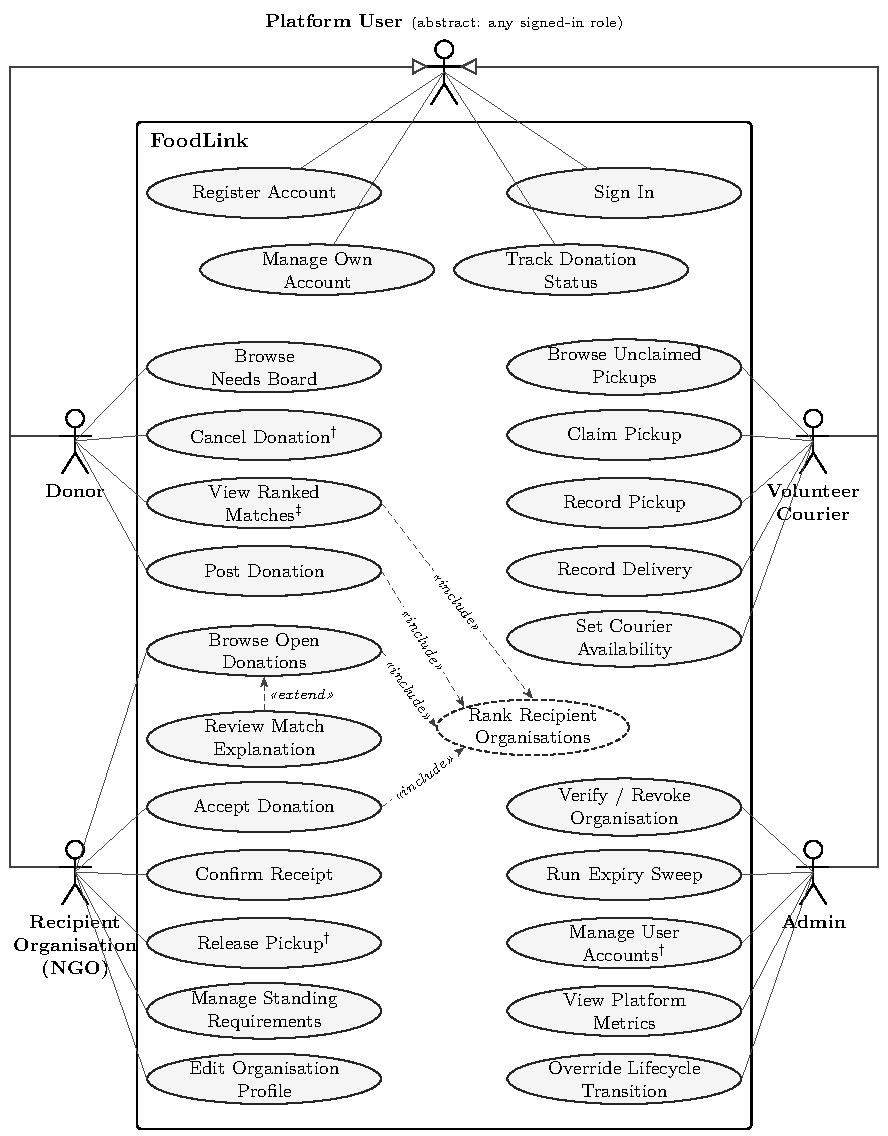
\includegraphics[width=\textwidth,height=0.9\textheight,keepaspectratio]{diagrams/use-case.pdf}
  \caption[Use case diagram of FoodLink]{Use case diagram of FoodLink.
    $\dagger$: implemented and tested in the API, not yet offered in the web
    portal. $\ddagger$: API and phone-layout camera screen only.}
  \label{fig:usecase}
\end{figure}

Figure~\ref{fig:usecase} shows four actors and 26 use cases. The actors
\emph{Donor}, \emph{Recipient Organisation (NGO)}, \emph{Volunteer Courier} and
\emph{Admin} specialise an abstract \emph{Platform User}, which carries sign-in,
account management and status tracking. \emph{Register Account} is open only to
the donor, organisation and courier roles. \emph{Post Donation}, \emph{View
Ranked Matches}, \emph{Browse Open Donations} and \emph{Accept Donation} each
$\ll$include$\gg$ the internal \emph{Rank Recipient Organisations}, and
\emph{Review Match Explanation} $\ll$extend$\gg$s \emph{Browse Open Donations}.
Some conditions are not drawn: browsing and accepting require a verified
organisation, overdue donations cannot be accepted, and donors cancel only
before pickup. \emph{Override Lifecycle Transition} represents the
administrator's place in every entry of \code{TRANSITION_ROLES} except the
courier claim.

\subsection{Use Case Scenarios}
\label{sec:scenarios}

The fifteen main use cases are specified below. Status codes are the server's
responses, and routes are relative to \code{/api}.

% ---------------------------------------------------------------------------
% A scenario is a ruled block of labelled fields; it may continue onto the
% next page. \flow numbers the main-flow steps inline.
\newcommand{\flow}[1]{\begin{enumerate*}[label=(\arabic*)]#1\end{enumerate*}}
\newenvironment{scenario}[2]{%
  \par\addvspace{8pt}\begingroup\small
  \noindent\rule{\linewidth}{0.4pt}\par\nopagebreak
  \noindent\textbf{#1 --- #2}\par\nopagebreak
}{%
  \par\endgroup
}
\newcommand{\ucfield}[2]{%
  \par\noindent\hangindent=2.5cm\hangafter=1%
  \makebox[2.5cm][l]{\textbf{#1}}#2\par}
% ---------------------------------------------------------------------------

\begin{scenario}{UC-01}{Register Account}
  \ucfield{Actor, goal}{Prospective donor, organisation or courier. \emph{Goal:} an account in a self-service role.}
  \ucfield{Pre., trigger}{Email unused; under 10 registrations per hour from the network. \emph{Trigger:} creating an account on the sign-in page.}
  \ucfield{Main flow}{\flow{\item Picks a role; enters name, email and password. \item \code{POST /auth/register} validates the email, an 8--128-character password and a self-signup role. \item The server stores a bcrypt hash and creates a courier or \emph{unverified} organisation profile. \item It returns 201 with a token.}}
  \ucfield{Alternatives}{Email exists: 409. \code{admin} role or invalid fields: 422. Over the limit: 429.}
  \ucfield{Post., rules}{Active account. An organisation is not ranked, cannot see the pool and cannot accept until verified (UC-13) and given coordinates (API only). Administrators never self-register (D-04).}
\end{scenario}

\begin{scenario}{UC-02}{Sign In}
  \ucfield{Actor, goal}{Any registered user. \emph{Goal:} an authenticated session in the right portal.}
  \ucfield{Pre., trigger}{Account exists; under 30 attempts per 5 minutes from the network. \emph{Trigger:} submitting email and password.}
  \ucfield{Main flow}{\flow{\item \code{POST /auth/login} (OAuth 2.0 password form). \item The server checks the bcrypt hash and that the account is active. \item It returns a 720-minute HS256 token, and the client opens the role's portal. \item Each later request re-reads the user.}}
  \ucfield{Alternatives}{Wrong email or password: 401 (one message). Suspended: 403. Over the limit: 429. Expired token or suspension mid-session: 401 and client sign-out.}
  \ucfield{Post., rules}{Signed in until expiry; sign-out is client-side. The token's role claim is never trusted (D-03).}
\end{scenario}

\begin{scenario}{UC-03}{Post Donation}
  \ucfield{Actor, goal}{Donor (or administrator). \emph{Goal:} offer surplus food to nearby verified organisations before it expires.}
  \ucfield{Pre., trigger}{Signed in; under 10 posts per hour for the account and 30 for the network. \emph{Trigger:} submitting \emph{Create Food Donation}.}
  \ucfield{Main flow}{\flow{\item Enters food details, address, pin, optional photo (resized in the browser) and deadline. \item \code{POST /donations} checks role, limits, field bounds and a future deadline. \item The donation is stored as \code{AVAILABLE} with an event, and organisations are ranked. \item If any is eligible, the top score is frozen and \code{MATCHED} recorded; 201 is returned.}}
  \ucfield{Alternatives}{None eligible: stays \code{AVAILABLE}. Past deadline or invalid input: 422. Over budget: 429. Organisation or courier: 403.}
  \ucfield{Post., rules}{Open to verified organisations until the deadline; nothing is assigned. Frozen score and distances are hidden from donors (D-47).}
\end{scenario}

\begin{scenario}{UC-04}{View Ranked Matches and Match Explanation}
  \ucfield{Actor, goal}{Recipient organisation; donor and administrator read the ranked list. \emph{Goal:} see how well a donation suits an organisation, and why.}
  \ucfield{Pre., trigger}{Organisation verified; donation open and not overdue. \emph{Trigger:} selecting a donation on \emph{Available Donations}, or \code{GET /donations/{id}/matches}.}
  \ucfield{Main flow}{\flow{\item \code{GET /donations} includes \code{viewerMatch}, the organisation's live \code{score_pair} result from its true position and own active needs. \item The panel shows the score, five sub-scores, distance and reasons. \item Variant: \code{/matches} lists up to 25 eligible organisations in order.}}
  \ucfield{Alternatives}{Unverified: pool not returned, with an explanation. Ineligible: no breakdown. Other readers: blurred positions, null \code{distanceKm}. Unreadable donation: 404.}
  \ucfield{Post., rules}{Read-only. Requirements affect only order and reasons (D-52); frozen and live scores differ (D-30).}
\end{scenario}

\begin{scenario}{UC-05}{Accept Donation}
  \ucfield{Actor, goal}{Recipient organisation (or an administrator for it). \emph{Goal:} take responsibility for an offered donation.}
  \ucfield{Pre., trigger}{Organisation verified; donation \code{AVAILABLE} or \code{MATCHED} and not overdue. \emph{Trigger:} \emph{Accept Donation}.}
  \ucfield{Main flow}{\flow{\item \code{POST /donations/{id}/status} with \code{ACCEPTED}. \item The server checks transition, role, deadline, own organisation and verification. \item It binds the organisation, counts one acceptance and freezes its score. \item The conditional write and event commit; the donation joins \emph{Accepted Deliveries} and the courier queue.}}
  \ucfield{Alternatives}{Overdue: 409. Unverified: 403. Another organisation accepted first: 409, changes rolled back. Another organisation's id: 403. No profile: 422.}
  \ucfield{Post., rules}{Exactly one bound organisation and one counted acceptance (D-06, D-50, D-55).}
\end{scenario}

\begin{scenario}{UC-06}{Claim Pickup}
  \ucfield{Actor, goal}{Volunteer courier. \emph{Goal:} take on collection and delivery.}
  \ucfield{Pre., trigger}{Courier profile exists; donation \code{ACCEPTED} and unclaimed. \emph{Trigger:} \emph{Accept Pickup} on \emph{Pickup Tasks}.}
  \ucfield{Main flow}{\flow{\item The queue shows food, deadline, organisation and only a coarse \code{pickupArea}. \item The courier requests \code{VOLUNTEER_ASSIGNED}. \item A conditional \code{UPDATE} binds the courier only if still \code{ACCEPTED} and unclaimed. \item The event commits; exact pin, address and donor become visible.}}
  \ucfield{Alternatives}{Another courier won: 409, ``Another courier has already claimed this pickup''. No longer \code{ACCEPTED}: 409. No courier profile: 422.}
  \ucfield{Post., rules}{Exactly one courier (D-28, D-57). Availability does not gate claiming; couriers are not verified.}
\end{scenario}

\begin{scenario}{UC-07}{Record Pickup and Delivery}
  \ucfield{Actor, goal}{The assigned courier. \emph{Goal:} record collection, then delivery.}
  \ucfield{Pre., trigger}{Donation \code{VOLUNTEER_ASSIGNED} to, or \code{PICKED_UP} by, the caller. \emph{Trigger:} \emph{Mark Picked Up}, then \emph{Mark Delivered}.}
  \ucfield{Main flow}{\flow{\item Sends \code{PICKED_UP}. \item The server checks transition and role and re-reads the donation through the courier's scope. \item The conditional write and event commit. \item \code{DELIVERED} follows the same way after handover.}}
  \ucfield{Alternatives}{Another courier's run: 404. Out of order: 409. After pickup the donor cannot cancel nor the organisation release (409).}
  \ucfield{Post., rules}{Awaits confirmation; in the courier's history from \code{DELIVERED} (D-51).}
\end{scenario}

\begin{scenario}{UC-08}{Confirm Receipt}
  \ucfield{Actor, goal}{The accepting organisation. \emph{Goal:} close the donation as received.}
  \ucfield{Pre., trigger}{Donation \code{DELIVERED} and bound to the caller. \emph{Trigger:} \emph{Confirm receipt} on \emph{Accepted Deliveries}.}
  \ucfield{Main flow}{\flow{\item Sends \code{COMPLETED}. \item The server checks transition, role and ownership. \item It increments the organisation's completions and the courier's deliveries. \item The conditional write and event commit.}}
  \ucfield{Alternatives}{Another organisation's donation: 404. Not yet delivered: 409. Donor or courier: 403.}
  \ucfield{Post., rules}{Terminal. Reliability updates for future rankings; counts towards the rescue rate if completed by the deadline.}
\end{scenario}

\begin{scenario}{UC-09}{Cancel Donation (API only)}
  \ucfield{Actor, goal}{Donor; secondary: administrator. \emph{Goal:} withdraw a donation that will not be handed over.}
  \ucfield{Pre., trigger}{Donor owns it and it is not yet \code{PICKED_UP} (an administrator may also cancel from \code{PICKED_UP}). \emph{Trigger:} status \code{CANCELLED} via the API; no portal button.}
  \ucfield{Main flow}{\flow{\item The server checks transition, role, ownership and the donor's window. \item The conditional write and \code{CANCELLED} event are applied. \item In the same transaction, a bound organisation's counted acceptance is withdrawn (never below zero).}}
  \ucfield{Alternatives}{Donor after pickup, or \code{DELIVERED}/\code{COMPLETED}: 409. Another donor: 404. A courier's pickup commits first: 409, nothing withdrawn.}
  \ucfield{Post., rules}{Terminal. Reliability is unaffected (D-58); no reason is recorded.}
\end{scenario}

\begin{scenario}{UC-10}{Release Pickup (API only)}
  \ucfield{Actor, goal}{The accepting organisation; secondary: administrator. \emph{Goal:} return a claimed pickup to the courier queue.}
  \ucfield{Pre., trigger}{Donation \code{VOLUNTEER_ASSIGNED} and bound to the caller's still-verified organisation. \emph{Trigger:} status \code{ACCEPTED} via the API; no portal button.}
  \ucfield{Main flow}{\flow{\item The server checks transition, role and ownership, treating this acceptance as a release. \item It confirms verification and the binding. \item It clears the courier without a new acceptance or re-frozen score. \item The conditional write and event commit.}}
  \ucfield{Alternatives}{Not the bound organisation: 404. Already picked up: 409. Verification revoked: 403.}
  \ucfield{Post., rules}{Unclaimed again, shown to couriers as a coarse area (D-41). Known issue: an administrator release naming another organisation counts a second acceptance.}
\end{scenario}

\begin{scenario}{UC-11}{Manage Standing Requirements and Browse Needs Board}
  \ucfield{Actor, goal}{Recipient organisation; secondary: donor. \emph{Goal:} publish needs before supply exists.}
  \ucfield{Pre., trigger}{Organisation profile exists (posting needs no verification). \emph{Trigger:} \emph{Food Requirements \& Demand Signals}; a donor opens \emph{Needs Board}.}
  \ucfield{Main flow}{\flow{\item \code{POST /requirements} with food type, quantity, unit, beneficiaries, urgency, recurrence and notes. \item \code{PATCH /requirements/{id}} edits or retires a need (\code{isActive: false}). \item Retired needs are listed with \code{includeInactive} and can be reopened. \item Donors see active needs of verified organisations.}}
  \ucfield{Alternatives}{Another organisation's id: 404. Invalid values: 422, nothing written. Explicit \code{null}: unchanged. Courier: empty list.}
  \ucfield{Post., rules}{Rows are never deleted. Active needs may break ties and add a reason, never change scores (D-29, D-44, D-52).}
\end{scenario}

\begin{scenario}{UC-12}{Edit Organisation Profile (verification-sensitive)}
  \ucfield{Actor, goal}{Recipient organisation. \emph{Goal:} keep the organisation's details correct.}
  \ucfield{Pre., trigger}{Organisation profile exists. \emph{Trigger:} saving \emph{NGO / Recipient Profile}.}
  \ucfield{Main flow}{\flow{\item \code{PATCH /recipients/me} with name, type, address, capacity, contact or phone. \item The server keeps real changes only; \code{null} clears only nullable fields. \item If a verified organisation's name, latitude or longitude changes, \code{is_verified} is cleared in the same commit. \item The page shows the result.}}
  \ucfield{Alternatives}{Non-positive capacity or out-of-range coordinates: 422. Unchanged name or other fields only: verification kept. Coordinates are API-only; clearing the pin voids verification.}
  \ucfield{Post., rules}{A voided organisation is excluded from ranking, pool and acceptance until re-verified (D-54); no self-verification (D-16).}
\end{scenario}

\begin{scenario}{UC-13}{Verify or Revoke Organisation}
  \ucfield{Actor, goal}{Administrator. \emph{Goal:} vouch for a genuine organisation, or withdraw that vouching.}
  \ucfield{Pre., trigger}{Signed in as administrator; organisation exists. \emph{Trigger:} the verify control on \emph{Partner Organizations Directory}.}
  \ucfield{Main flow}{\flow{\item The page lists organisations with verification state, reliability and the number awaiting verification. \item After checking outside the system, the administrator sends \code{POST /admin/recipients/{id}/verify}. \item The server sets \code{is_verified}; the list refreshes. \item \code{DELETE} on the same route revokes.}}
  \ucfield{Alternatives}{Non-administrator: 403. Unknown organisation: 404.}
  \ucfield{Post., rules}{Verified with coordinates: ranked, sees the pool, can accept; revoked: loses these, accepted donations unaffected. Verification is a human judgement (D-37); administrator-created organisations start verified.}
\end{scenario}

\begin{scenario}{UC-14}{Run Expiry Sweep}
  \ucfield{Actor, goal}{Administrator. \emph{Goal:} record unaccepted, overdue donations as losses.}
  \ucfield{Pre., trigger}{Signed in as administrator. \emph{Trigger:} running the sweep from \emph{Platform Donation Ledger}.}
  \ucfield{Main flow}{\flow{\item \code{POST /admin/maintenance/expire}. \item The server selects \code{AVAILABLE} and \code{MATCHED} donations past their deadline. \item It appends actor-less \code{EXPIRED} events (``Deadline passed with no recipient'') and sets the status. \item It returns the count.}}
  \ucfield{Alternatives}{Nothing overdue: count 0. Non-administrator: 403.}
  \ucfield{Post., rules}{Terminal; counted in the expiry-loss rate. Known issues: not scheduled, overdue \code{ACCEPTED} donations untouched, write not conditional.}
\end{scenario}

\begin{scenario}{UC-15}{Manage User Accounts (API only)}
  \ucfield{Actor, goal}{Administrator. \emph{Goal:} create accounts of any role; suspend, restore, rename or re-role them.}
  \ucfield{Pre., trigger}{Signed in as administrator. \emph{Trigger:} calls to \code{/admin/users}; no screen.}
  \ucfield{Main flow}{\flow{\item \code{GET} lists accounts, optionally by role. \item \code{POST} creates any role, including administrator, with its profile (organisations start verified). \item \code{PATCH /admin/users/{id}} updates \code{isActive}, \code{role}, \code{name}, \code{organization} or \code{phone}.}}
  \ucfield{Alternatives}{Duplicate email: 409. Suspending or demoting oneself or the last active administrator: 409. Unknown user: 404.}
  \ucfield{Post., rules}{Effective on the next request (a suspended user receives 401, and 403 at sign-in). The first administrator comes only from \texttt{python -m foodlink.cli create-admin} (D-04).}
\end{scenario}

\medskip
\noindent The remaining use cases in Figure~\ref{fig:usecase} are simple.
\emph{Manage Own Account} uses \code{PATCH /auth/me} and
\code{POST /auth/password}; \emph{Track Donation Status} lists donations in
one's scope with their timelines; \emph{Browse Unclaimed Pickups} is the
coarse-area queue of UC-06; \emph{Set Courier Availability} uses
\code{PATCH /volunteers/me} and is advisory; \emph{View Platform Metrics} calls
\code{GET /metrics}; and \emph{Override Lifecycle Transition} performs any
transition in Table~\ref{tab:transitions} except the claim, on a party's behalf.

\section{Class Diagram}
\label{sec:class}

\begin{figure}[p]
  \centering
  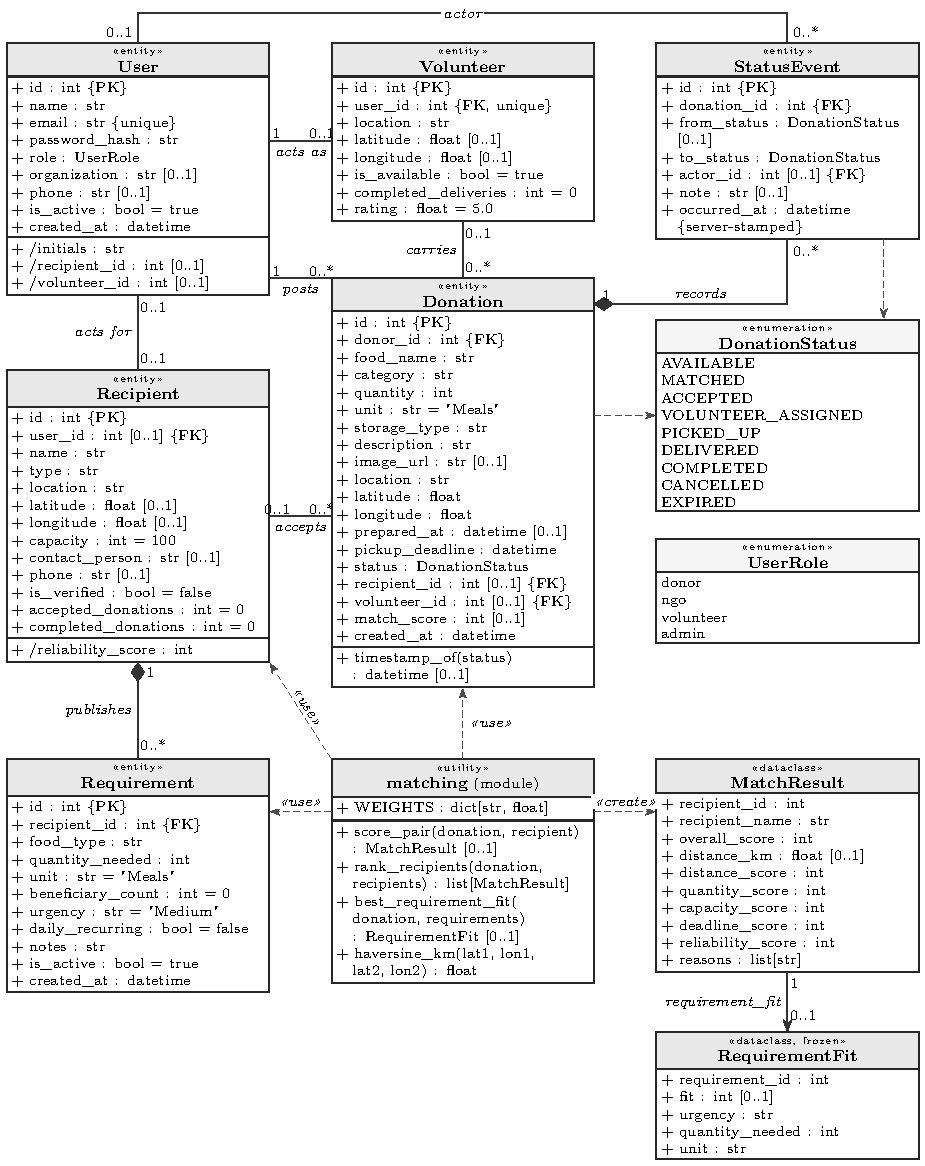
\includegraphics[width=\textwidth,height=0.9\textheight,keepaspectratio]{diagrams/class-diagram.pdf}
  \caption{Class diagram of the FoodLink domain model and matching module}
  \label{fig:class}
\end{figure}

Figure~\ref{fig:class} shows the six persistent entities and two enumerations
of \code{models.py}, and the \code{matching} module with its two data classes.
Multiplicities follow the foreign keys: a user acts for at most one
\code{Recipient} (seeded recipients have none) and at most one \code{Volunteer},
whose user key is unique and mandatory; a \code{Donation} has zero or one
recipient and courier until acceptance and claim; and a \code{StatusEvent}
optionally names its actor. \code{Donation}--\code{StatusEvent} and
\code{Recipient}--\code{Requirement} are compositions with cascading deletes,
and derived properties carry a slash (for example
\code{Recipient.reliability_score}). The matching module is a
$\ll$utility$\gg$ whose \code{MatchResult} objects are transient; only
\code{overall_score} is copied into \code{Donation.match_score}. Roles are an
enumerated attribute and profiles are associations, so there is no inheritance.

\section{Activity Diagram}
\label{sec:activity}

\begin{figure}[p]
  \centering
  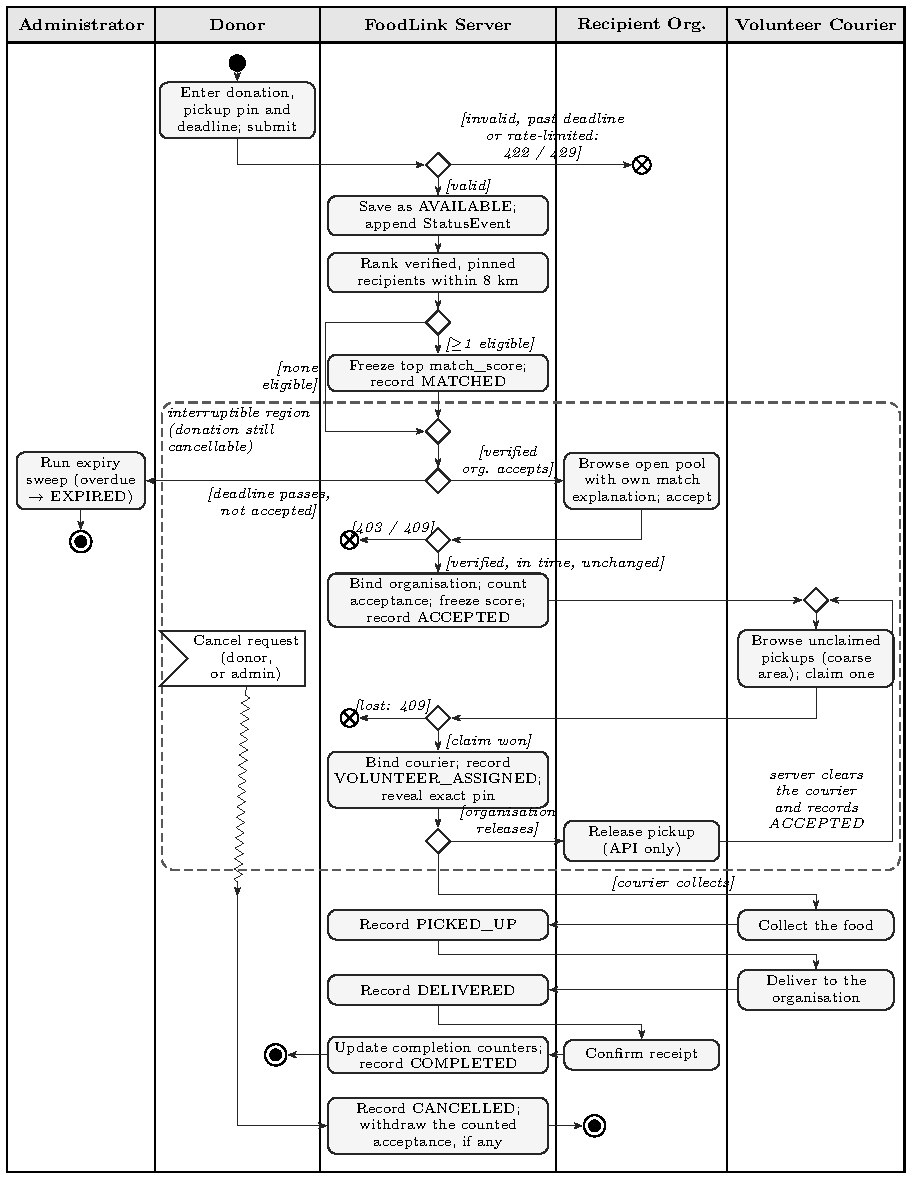
\includegraphics[width=\textwidth,height=0.9\textheight,keepaspectratio]{diagrams/activity-diagram.pdf}
  \caption[Activity diagram of the donation lifecycle]{Activity diagram of the
    donation lifecycle, from posting to completion, expiry or cancellation.
    Codes on refusal edges: 422 invalid input or past deadline; 429 rate
    limit; 403 unverified organisation; 409 overdue, already taken or claim
    lost.}
  \label{fig:activity}
\end{figure}

Figure~\ref{fig:activity} models the workflow across five swimlanes: the four
roles and the server, the only lane that records state. The main path runs
through validation, storage and ranking (\code{MATCHED} only when an
organisation is eligible), acceptance gated by verification, the deadline and a
conditional write, then a conditional courier claim, pickup, delivery and
confirmation. Refused requests end at flow-final nodes and leave the donation
unchanged. Donations nobody accepts in time end in \code{EXPIRED} through the
sweep, and an API-only release loop returns a claimed pickup to the queue. The
dashed interruptible region spans the states in which a donor may still cancel;
its interrupting edge ends in \code{CANCELLED} and withdraws any counted
acceptance. Administrator cancellation after pickup, administrator
\code{ACCEPTED}\,$\to$\,\code{EXPIRED}, and administrators acting for other
parties are omitted for readability.


% ===== BIBLIOGRAPHY =====

% Print bibliography with heading in TOC
\printbibliography[heading=bibintoc]

\end{document}
